% ----------- Document settings -----------
\documentclass[nonacm, sigconf, balance=true]{acmart}
% ====================================================
% General layout, typography & document-wide settings
% ====================================================

% ----------- Document settings -----------
\def\documentTitle      {Onderzoeken schrijven in Latex} % replace with actual document title
\def\documentSubtitle   {Een basis bestand voor een gelijke uitstraling} % replace with actual subtitle if any, else leave empty
\def\authorName         {John Doe} % replace with actual author name
\def\authorEmail        {JohnDoe@gmail.com} % replace with actual author email
\def\institutionName    {Harvard} % replace with actual institution name
\def\institutionCountry {Verenigde Staten} % replace with actual institution location
\def\institutionCity    {Massachusetts} % replace with actual institution location
\def\dueDate            {Oktober 2025} % replace with actual due date

\def\editorsVersion     {false} % true om editorsnote e.d. te tonen, false voor verbergen
\def\makeTitlePage      {true}  % true om titelpagina te maken, false om over te slaan
\def\makeTOCpage        {true}  % true om inhoudsopgave te maken, false om over te slaan

\def\listMark           {-} % itemize marker, e.g. '-', '*', '\textbullet', etc.

%----------- DONT TOUCH BELOW THIS LINE -----------
\usepackage{xparse}
\usepackage{xstring}

% ----------- Encoding & Fonts -----------
\usepackage[T1]{fontenc}
\usepackage[utf8]{inputenc}
\usepackage{scalefnt}

% ----------- Page layout -----------
\usepackage{expl3}
\usepackage{array}
\setlength{\columnsep}{0.333in}
\renewcommand{\baselinestretch}{1.05}
\setlength\parindent{2mm}
\setlength{\footskip}{40pt} %set footer size bigger to avoid overlap with text
\usepackage{geometry}
\geometry{
    a4paper,
    left=15mm,
    right=15mm,
    top=15mm,
    bottom=15mm,
}

% ----------- Table of Contents -----------
\usepackage{titletoc}
\setcounter{tocdepth}{2} % include subsections in TOC
%
 \titlecontents{section}
 [0] % i
 {\vspace{0.05cm}}
 {\thecontentslabel\enspace}%\thecontentslabel
 {}
 {\titlerule*[0.1cm]{.}\contentspage}%]

 \titlecontents{subsection}
 [1em] %
 {\vspace{0.05cm}}
 {\thecontentslabel\enspace}%\thecontentslabel
 {\hspace*{1em}}
 {\titlerule*[0.1cm]{.}\contentspage}


% ----------- Typography -----------
\usepackage{microtype} % subtle spacing & justification improvements

% ----------- Headings -----------
\usepackage{titlesec}
\titleformat{\section}{\large\bfseries}{\thesection}{1em}{}
\titleformat{\subsection}{\normalsize\bfseries}{\thesubsection}{0.75em}{}

% ----------- Lists -----------
\usepackage{enumitem}
\setlist[itemize]{
    leftmargin = *,
    listparindent = 10mm,
    label = {\listMark} % makes the default item marker a dash
}

% ----------- Figures & Tables -----------
\usepackage{graphicx}
\usepackage{subcaption}
\usepackage{tcolorbox}
\usepackage{float}
\usepackage{tabularx}
\usepackage{booktabs} % professional tables
\usepackage[table]{xcolor}
\usepackage{environ}

% Caption formatting
\usepackage{caption}
\captionsetup[table]{
    name=Tabel,                  % rename "Table" to "Tabel"
    labelfont={bf},              % "Tabel 1:" in bold
    textfont={normalfont},       % caption text in normal (non-bold)
    labelsep=colon               % ensures "Tabel 1:" (with colon)
}

\captionsetup[figure]{
    name=Figuur,                 % rename "Figure" to "Figuur"
    labelfont={bf},              % "Figuur 1:" in bold
    textfont={normalfont},       % caption text in normal (non-bold)
    labelsep=colon               % ensures "Figuur 1:" (with colon)
}

% ----------- Footnotes -----------
\usepackage[hang,flushmargin]{footmisc}

% ----------- Hyperlinks -----------
\usepackage[
    colorlinks=true,
    linkcolor=blue,
    citecolor=blue,
    urlcolor=blue,
]{hyperref}

% ----------- Column balance -----------
\usepackage{balance}

% ----------- Bibliography -----------
\usepackage[backend=biber,style=apa]{biblatex}
\DeclareLanguageMapping{dutch}{dutch-apa}
\DefineBibliographyStrings{dutch}{andothers = {et al.}}
\addbibresource{main.bib}
\setlength\bibitemsep{0.25em}

% ----------- ACM-style tweaks (optional) -----------
\settopmatter{printacmref=false}
\setcopyright{none}
\settopmatter{printfolios=true}
\renewcommand\footnotetextcopyrightpermission[1]{}

% ----------- Editors/general version -----------
\usepackage{comment}
\usepackage{ifthen}
\newboolean{editorsversion}
\setboolean{editorsversion}{\editorsVersion}  % change to false for student version


% ----------- Paper layout information -----------
\title{\documentTitle}
\subtitle{\documentSubtitle}

\author{\authorName}
\date{\dueDate}
\email{\authorEmail}
\affiliation{
    \institution{\institutionName}
    \city{\institutionCity}
    \country{\institutionCountry}
}

\hypersetup{
    pdfauthor={\authorName},
    pdftitle={\documentTitle},
    pdfborder={0 0 0}
}

% When \begin{document} is written, also add \maketitle and \tableofcontents there. (if settings are true)
\AtBeginDocument
{%
    \ifthenelse{\equal{\makeTitlePage}{true}}{%
        \maketitle
    }{}
    \ifthenelse{\equal{\makeTOCpage}{true}}{%
        \tableofcontents
        \newpage
    }{}
}% % import custom general paper settings
% --------------------------------
% This file contains a custom set
% of commands to make writing
% LaTeX easier
% --------------------------------

% makes 0.05 inches of horizontal space
\newcommand{\vertspace}{\vspace{0.05in}}

% writes centered italic text 80% width of the page/column and gives top & bottom padding
\newcommand{\question}[1]{\vertspace\begin{center}\parbox{0.8\linewidth}{\centering\textit{#1}}\end{center}\vertspace}

% Writes a single paragraph of Lorum Ipsum text
\newcommand{\lorem}{Lorem ipsum dolor sit amet, consectetur adipiscing elit. Nullam eget tortor a urna ornare pellentesque. Integer sit amet purus nec sem iaculis euismod. Duis at ipsum eu libero pharetra egestas. Quisque eleifend odio velit, at sollicitudin metus dictum eu. Integer nec mi congue, gravida nibh sed, faucibus mauris. Sed vel ipsum lobortis felis gravida dignissim. Curabitur vestibulum turpis eu orci lacinia consectetur.}

% APA style qoutes
\usepackage{xstring}
\newcommand{\qoute}[3]{%
  % Count the number of words in the quote
  \StrCount{#1}{ }[\woordenaantal]%
  \ifthenelse{\woordenaantal < 39}{``\textit{#1}'' (\citeauthor{#2}, \citeyear{#2}, p. #3)}% Kort citaat (minder dan 40 woorden)
  {
    \vertspace
    \begin{flushright}
      \parbox{0.95\linewidth}{\textit{#1}}
      (\citeauthor{#2}, \citeyear{#2}, p. #3)
    \end{flushright}
    \vertspace % Lang citaat (40 woorden of meer)
  }
}

% cites like \parencite[prenote][postnote]{cite}
\newcommand{\parencite}[3][]{%
    (#1 \citeauthor{#3}, \citeyear{#3}#2)%
}



% command for Editor's notes and comments
% defines custom commands:
% - \editorsonly{...} for inline comments
% - \begin{editorsonlyBox} ... \end{editorsonlyBox} for boxed comments
% - \editorsfootnote{...} for comments in footnotes
\ifthenelse{\boolean{editorsversion}}{%
    % EDITORS VERSION
    % inline red comments - compact, no paragraph indentation
    \newcommand{\editorsonly}[1]{%
        \par\vspace{0.05in}
        {\footnotesize\noindent\textcolor{red!70!black}{\textbf{Editor's note:} #1}}%
        \par\vspace{0.05in}
    }

    % environment for soft-background editor comments
    \newenvironment{editorsonlyBox}{%
        \par\medskip
        \begin{tcolorbox}[
            enhanced,
            breakable,
            colback=red!5,
            colframe=red!20!white,
            boxrule=0pt,
            borderline north={1pt}{0pt}{red!40!white},
            sharp corners,
            before skip=6pt,
            after skip=6pt,
            title={\textcolor{red!60!black}{\footnotesize Comment for editors:}},
            coltitle=red!70!black,
            fonttitle=\bfseries,
            top=2pt,
            bottom=2pt,
            left=4pt,
            right=4pt
        ]
    }{%
        \end{tcolorbox}
    }

    % red footnotes for editors
    \newcommand{\editorsfootnote}[1]{%
        \textcolor{red!70!black}{\footnote{\textcolor{red!70!black}{Editor's note: #1}}}%
    }

    % command to cite all references in the .bib file (for editors only)
    \nocite{*}
}{%
% STUDENT VERSION: suppress all editor content
    \newcommand{\editorsonly}[1]{\ignorespaces}
    \newenvironment{editorsonlyBox}{\comment}{\uncomment}
    \newcommand{\editorsfootnote}[1]{}
}

%%% ---------- TEXT SPLITTER ----------
%    The \splittext{<text>}{<n>} command splits <text> into lines of maximum <n> characters.
%    It inserts a line break (\\) every n characters.
%
%    Example usage:
%    \splittext{This is an example of splitting text into multiple lines every n characters.}{10}
%
%    This will produce:

\ExplSyntaxOn
\NewDocumentCommand{\spliteveryn}{mm}
 {
  % #1 = number of characters per line
  % #2 = text to split
  \str_set:Nn \l_tmpa_str { #2 }
  \int_zero:N \l_tmpa_int
  \str_map_inline:Nn \l_tmpa_str
   {
       ##1
       \int_incr:N \l_tmpa_int
       \int_compare:nNnT { \l_tmpa_int } = { #1 }
           {
           \\
           \int_zero:N \l_tmpa_int
       }
   }
 }
\ExplSyntaxOff

% --- Helper macro to check if argument is empty ---
\makeatletter
\newcommand{\IfNonEmpty}[2]{%
    \if\relax\detokenize{#1}\relax
    % empty → do nothing
    \else
    #2%
    \fi
}
\makeatother


%%% ---------- TABLE MACROS ----------
%    To use the SimpleTable command, use the following format:
%    \SimpleTable{<caption>}{<label>}{%
%        \TableRow{<Aspect 1>}{<Description 1>}
%        \TableRow{<Aspect 2>}{<Description 2>}
%        ...
%    }
%
%    Example usage:
%
%    \SimpleTable
%    {Overzicht van de belangrijkste elementen uit \textit{Smart Doorbell Security System Using IoT}.}
%    {tab:doorbell}
%    {
%        \TableRow{Probleemstelling}{Bestaande beveiligingssystemen vertrouwen enkel op gezichtsherkenning; onbekende gezichten worden niet gecontroleerd of gemeld.}
%        \TableRow{Doel van het systeem}{Ontwikkelen van een slimme deurbel die gebruikmaakt van IoT, gezichtsherkenning, stemherkenning en bewegingsdetectie om bezoekers automatisch te identificeren.}
%        \TableRow{Werking}{Bij het aanbellen activeert de Raspberry Pi een camera; de foto wordt vergeleken met een database van geregistreerde gezichten. Onbekende bezoekers leiden tot een e-mailmelding met foto en OTP naar de eigenaar.}
%        \TableRow{Technologieën}{Raspberry Pi, OpenCV (beeldverwerking), DSP (stemherkenning), Speech-to-Text, e-mailserver voor OTP-verzending.}
%    }
% --- Table Header + Row commands ---
\NewDocumentCommand{\TableHeader}{m m}{%
    \arrayrulecolor{black!80}\specialrule{1pt}{0pt}{2pt}
    \textbf{#1} & \textbf{#2} \\ \midrule
}
\NewDocumentCommand{\TableHeaderThree}{m m m}{%
    \arrayrulecolor{black!80}\specialrule{1pt}{0pt}{2pt}
    \textbf{#1} & \textbf{#2} & \textbf{#3} \\ \midrule
}

\NewDocumentCommand{\TableRow}{m m}{%
    \textbf{#1} & #2 \\ \arrayrulecolor{black!10}\specialrule{0.5pt}{1pt}{0pt}\arrayrulecolor{black!100}
}
\NewDocumentCommand{\TableRowThree}{m m m}{%
    #1 & #2 & #3 \\ \arrayrulecolor{black!10}\specialrule{0.5pt}{1pt}{0pt}\arrayrulecolor{black!100}
}


% --- Updated 2-column version ---
\newcommand{\SimpleTableTwo}[3]{%
    \begin{table}[h!]
        \centering
        \scalefont{0.75}%
        \resizebox{\columnwidth}{!}{%
            \begin{tabular}{@{}p{0.25\linewidth}p{0.70\linewidth}@{}}

                #3
                \arrayrulecolor{black!80}\specialrule{1pt}{0pt}{2pt}
            \end{tabular}%
        }%
        \scalefont{1}%
        \IfNonEmpty{#1}{\caption{#1}}%
        \IfNonEmpty{#2}{\label{#2}}%
    \end{table}%
}

% --- Updated 3-column version ---
\newcommand{\SimpleTableThree}[3]{%
    \begin{table}[h!]
        \centering
        \scalefont{0.75}%
        \resizebox{\columnwidth}{!}{%
            \begin{tabular}{@{}p{0.33\linewidth}p{0.33\linewidth}p{0.33\linewidth}@{}}
                \arrayrulecolor{black!80}\specialrule{1pt}{0pt}{2pt}
                #3
                \arrayrulecolor{black!80}\specialrule{1pt}{0pt}{2pt}
            \end{tabular}%
        }%
        \scalefont{1}%
        \IfNonEmpty{#1}{\caption{#1}}%
        \IfNonEmpty{#2}{\label{#2}}%
    \end{table}%
}

% --- Smart dispatcher: decides between 2 or 3 cols automatically ---
\NewDocumentCommand{\SimpleTable}{m m m}{%
    \IfSubStr{#3}{\TableHeaderThree}{%
        \SimpleTableThree{#1}{#2}{#3}%
    }{%
        \SimpleTableTwo{#1}{#2}{#3}%
    }%
}
 % import custom commands and packages

% ----------- Start document -----------

\begin{document}
    \section{abstract}
    Er verschijnen steeds meer videodeurbellen aan de deurposten.
    Dit roept de vraag op of dit niet een immense inbreuk op privacy is.
    Het doel van dit onderzoek is om te achterhalen of en hoe privacy in de verdrukking komt door deze nieuwe surveillancetrend.
    De achterliggende onderzoeksvraag is daarom ook: \textit{Hoe beïnvloedt het constant filmen van slimme deurbellen de privacy van buren en voorbijgangers?}
    Om op een antwoord te komen wordt er een bronnenonderzoek gedaan en worden de bevindingen op verschillende gebieden \hyperref[subsec:privacy-theorie]{\textbf{Privacy theorie}}, \hyperref[subsec:technische-aspecten-van-slimme-deurbellen]{\textbf{technische aspecten van slimme deurbellen}}, \hyperref[subsec:maatschappelijke-en-ethische-implicaties]{\textbf{maatschappelijke en ethische implicaties}} en \hyperref[subsec:gebruikerservaring-/-gedrag2]{\textbf{gebruikerservaringen / gedrag}}

    Uit de bronnen blijkt dat de bedrijven die achter de videodeurbellen zitten, niet altijd het beste voor hebben met de klanten.
    Ook is het niet altijd duidelijk wat er met de data gebeurt die wordt opgenomen door de deurbellen en/of ze daadwerkelijk verwijderd worden als dat gevraagd is.
    Maar niet alles is aan de bedrijven te wijten, want klanten (met name ``ervaren gebruikers'') hadden liever gemak en functies over privacy.


    \section{Introductie}
    We leven in een tijd waarin zoveel mogelijk onderdelen van iemands leven aan het internet gekoppeld (kunnen) worden.
    Zo ook je eigen voordeur: de opkomst van zogenaamde videodeurbellen, zoals deurbellen van Ring of Eufy, is een steeds bekender gezicht in de wijken van Nederland.
    Het plus- (en tevens ook min-)punt van deze producten is dat elke (verdachte) beweging die de deurbel detecteert, wordt opgenomen en doorgestuurd naar de eigenaar.
    Mogelijke inbrekers worden afgeschrikt door het idee dat ze op video staan bij een inbraakpoging en dat zorgt bij veel mensen voor een veilig gevoel, maar dit heeft ook een keerzijde.
    De postbode die je krantje komt bezorgen, maar ook voorbijrijdende auto's, buren die een ommetje maken of kinderen die langsfietsen worden ook opgenomen, terwijl dit niet de doelgroep is waarvoor (of waartegen) deze deurbel ontworpen is.
    Dit roept de vraag op:

    \question{Hoe beïnvloedt het constant filmen van slimme deurbellen de privacy van buren en voorbijgangers?}

    Deze vraag sluit nauw aan bij het concept contextuele integriteit van Helen Nissenbaum, waarin iemand zo goed mogelijk in zijn of haar persoonlijke vrijheid gelaten wordt en data alleen in een passende context gedeeld mag worden.
    Videodeurbellen doorbreken deze verwachte informatiestromen, want waar voorbijgangers normaal anoniem over straat liepen, worden zij nu onbewust onderdeel van een digitaal surveillancesysteem.


    \subsection{Theoretisch kader}

    \parencite{nissenbaum2009privacy} Schreef al over een door haar ontwikkeld privacy theorie: \textbf{contextuele integriteit}.
    Dit schreef zij in haar boek \textit{Privacy In Context: Technology, Policy, and the Integrity of Social Life.}

    \vsmall
    \begin{itemize}
        \item Privacy wordt gewaarborgd door passende informatiestromen.
        \item Passende informatiestromen zijn stromen die voldoen aan contextuele informatienormen.
        \item Contextuele informatienormen verwijzen naar vijf onafhankelijke parameters: betrokkene, afzender, ontvanger, informatietype en transmissie-principe.
        \item Concepties van privacy zijn gebaseerd op ethische overwegingen die in de loop der tijd evolueren.
    \end{itemize}
    \vsmall

    \citeauthor{nissenbaum2009privacy} stelt dat privacy en wat acceptabel is om te delen af hangt van de situatie waarin men op dat moment leeft.
    Een voorbeeld hiervan is dat het (doorgaans vaak) niet gewenst is om je medische dossier met Jan en alleman te delen, echter met een dokter of huisarts is dit natuurlijk wel wenselijk.
    Hier komt contextuele integriteit goed naar boven.
    Want gebaseerd op de situatie deel je (of wil je) wel of niet bepaalde data met bepaalde entiteiten en deze entiteiten deze data ook niet doorgeven aan andere waarvoor de data niet nodig is.

    Dit wijkt af van het ``traditionele" denkbeeld, oftwel \textit{control over information} waarin een individu zelf zijn data beheert en kiest of data wel of niet gedeeld wordt.
    Dit is veel meer individu-gecentreerd en contextuele integriteit is meer (je raadt het al) context-gecentreerd.

    \subsection{Relevantie}
    Videodeurbellen zijn dus nauw verbonden met het concept contextuele integriteit.
    Voor eigen veiligheid (of gemoedsrust) schaffen steeds meer mensen een videodeurbel aan, dit gaat echter ten koste van de privacy van voorbijgangers, buren en andere die toevallig langs een huis met een videodeurbel lopen.
    Daarom wordt in dit onderzoek gekeken naar of de waarde in veiligheidsgevoel opweegt tegen het ongevraagd (en passief) filmen van voorbijgangers en dergelijke.


    \section{Methode}
    Dit onderzoek is een kwantitatief onderzoek om de vragen rondom de contextuele integriteit en privacy en Slimme (video) deurbellen te beantwoorden.
    Hiervoor is uitsluitend literatuuronderzoek gedaan.
    Er zijn veel verschillende bronnen geraadpleegd, dit is grotendeels via Google Scholar gedaan.
    Hierbij zijn verschillende zoektermen gebruikt zoals: Slimme deurbel, Ring (video)deurbel, Smart doorbell, Privacy video doorbell.

    De gebruikte bronnen zijn afkomstig uit wetenschappelijke publicaties en tijdschriften.
    Zo vormt het werk van \citeauthor{nissenbaum2009privacy} een theoretisch fundament op het gebied van privacy en contextuele integriteit.

    \citeauthor{van2016privacy} biedt een bruikbaar framework en \citeauthor{shaffer2021applying} levert een casestudy over de samenwerking tussen Ring en de politie, wat direct aansluit bij het onderwerp van dit onderzoek~(\ref{subsec:privacy-theorie}).
    Daarnaast bieden studies van \citeauthor{liu2021ethical}, \citeauthor{lalitha2019smart} en \citeauthor{chaudhari2020smart} een technisch perspectief op slimme deurbellen, waarbij veiligheid en functionaliteit empirisch worden onderzocht~(\ref{subsec:technische-aspecten-van-slimme-deurbellen}).
    Tot slot leveren \citeauthor{selinger2022amazon} en \citeauthor{kelly2023ring} kritische beschouwingen over Amazon's Ring en de maatschappelijke gevolgen van consumentgestuurde surveillance~(\ref{subsec:maatschappelijke-en-ethische-implicaties}).
    Artikelen van \citeauthor{shaffer2021applying} en \citeauthor{tabassum2023exploring} bouwen daarop voort met recente analyses van smart home-privacy en gebruikerscontrole, gepubliceerd in peer-reviewed journals~(\ref{subsec:gebruikerservaring-/-gedrag2}).
    Samen bieden deze bronnen een goed gebalanceerde mix van theoretische, technische en ethische invalshoeken, afkomstig uit betrouwbare en actuele academische contexten.


    \section{Beschouwing van literatuur}

    \subsection{Privacy-theorie}\label{subsec:privacy-theorie}
    \parencite{van2016privacy} stelt dat data in een privacy framework (Figuur~\ref{fig:privacy_framework}) opgedeeld kan worden.
    Deze is opgedeeld in twee assen: de y-as geeft aan of data wel of niet persoonlijk is, en de x-as geeft aan of data wordt gebruikt om te helpen of om te monitoren.

    \begin{figure}[h]
        \centering
        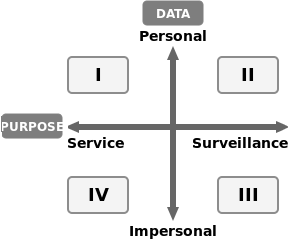
\includegraphics[width=40mm]{images/SmartCityPrivacy}
        \caption{Privacy framework {\prepostparencite[nagemaakt van][]{van2016privacy}}}
        \label{fig:privacy_framework}
    \end{figure}

    In het tweede kwadrant (\textbf{II}) gaat het over het verzamelen van persoonlijke data om te monitoren.
    Dit betreft bijvoorbeeld politiedata of beelden van beveiligingscamera's.
    Mensen ervaren dit als zeer persoonlijke en gevoelige informatie, wat tot kritiek leidt op toezicht en controle.
    Zo kreeg de burgemeester van Nice in 2008 een "Big Brother Award" voor het volhangen van de stad met camera's, en Dresden kreeg deze prijs in 2012 voor het volgen van mobiele telefoons tijdens een demonstratie.

    Tegelijkertijd hangt hoe bezorgd mensen af van tijd en situatie.
    Zo werd geschreven:
    \uitspraak{Acceptance of the US government monitoring personal communications was high in the immediate aftermath of the 9/11 attacks but declined after about half a year.}{van2016privacy}{474}

    Het derde kwadrant (\textbf{III}) gaat over data die niet direct aan één persoon gekoppeld zijn, maar wél gebruikt worden om gedrag of situaties te controleren.
    Denk aan verkeersstromen of drukte op stations en evenementen.
    Op het eerste gezicht lijkt dit onschuldig, omdat het om groepen, patronen of cijfers gaat, en niet om individuen.

    Steden gebruiken zulke "anonieme" data vaak om beleid te maken.
    Rotterdam bijvoorbeeld verzamelt en koppelt diverse datasets, van politiedata tot economische cijfers, om risicowijken te identificeren of criminaliteit te voorspellen\footnote{Ook wel \textit{predictive policing} genoemd}.
    Toch schuilt hier een gevaar: hoe meer datasets worden gekoppeld, hoe makkelijker het wordt om individuen te identificeren.
    Anonieme data verandert zo in persoonlijke data, wat wantrouwen en zorgen over discriminatie en controle kan veroorzaken.

    Een concreet voorbeeld van deze privacyzorgen is de samenwerking tussen Ring en de Long Beach Police Department (LBPD) in augustus 2019~\parencite{shaffer2021applying}.
    Via de app \textit{Neighbors} konden bewoners videobeelden van Ring-deurbellen delen met de politie.
    Officieel vrijwillig, maar in de praktijk voelde het voor velen als een sluiproute naar burgerlijke surveillance.
    De reacties waren gemengd: sommigen zagen het als logisch voor criminaliteitsbestrijding, anderen als zorgelijk omdat politie en een commercieel bedrijf (Amazon, het moederbedrijf van Ring) steeds dieper in de privésfeer doordringen.
    Het ongemak werd versterkt doordat bewoners Amazon veel minder vertrouwen dan de politie.

    Uiteindelijk draait de discussie niet om de videodeurbellen zelf, maar om macht en controle: wie kijkt mee, en wie bepaalt wat er met de verzamelde data gebeurt?

    \subsection{Technische aspecten van slimme deurbellen}\label{subsec:technische-aspecten-van-slimme-deurbellen}
    Een samengevoegd overzicht van technische, bouwkundige en praktische perspectieven op privacy en beveiliging bij slimme deurbellen.
    Hieronder volgen de bevindingen en reflecties uit drie studies — elk met hun eigen focus — maar samengebracht onder één overkoepelend thema: wat betekent \emph{privacy} technisch en praktisch in een world-wide-netwerk van videodeurbellen?

    Na uitvoerig \textit{threat modeling} en \textit{penetration testing} concludeert~\parencite{liu2021ethical} dat de onderzochte smart video deurbel over het algemeen degelijk maar niet foutloos is.
    Er werden geen directe, kritieke zero-days\footnote{Een beveiligingsprobleem dat nog geen oplossing heeft en nog niet bekend is bij de ontwikkelaars} gevonden, maar er zijn meerdere zwakke plekken die in de praktijk misbruikt kunnen worden — met name in de Android-app, de accountbeveiliging en de draadloze communicatie.
    Belangrijk is dat deze zwaktes vooral aantonen dat privacy geen gegeven is; het is iets dat voortdurend verdedigd moet worden.

    % 2 columns
    \begin{SimpleTable}[s{0.5}s{1.5}]{Overzicht van de belangrijkste beveiligingsbevindingen van de smart video deurbel}{tab:doorbell-findings}
        \TableHeader{Categorie & Belangrijkste bevindingen en verbeterpunten}
        \TableRow{Android-applicatie & Gevoelige data kan uitlekken doordat de app-data niet goed wordt afgeschermd. Externe opslag moet worden vermeden en verouderde encryptie vervangen, certificaatvalidatie is zwak (zelfondertekende certificaten worden te snel vertrouwd). Positief is dat de code lastig te manipuleren is door de gesegmenteerde .dex-bestanden.}
        \TableRow{Accountbeveiliging & Wachtwoorden worden gehasht met MD5, wat onveilig is en makkelijk te breken. Sessies worden in URL's doorgegeven in plaats van via veilige cookies of POST-methoden. CAPTCHA's beperken brute-force aanvallen effectief en het wachtwoordbeleid zorgt voor goed genoege wachtwoorden.}
        \TableRow{Draadloze communicatie & Verkeer tussen app en deurbel verloopt via HTTPS, waardoor afluisteren bemoeilijkt wordt. Toch blijft een MitM-aanval mogelijk als de aanvaller een eigen CA weet te installeren. Replay-aanvallen zijn theoretisch uitvoerbaar bij specifieke verzoeken (zoals uitloggen of gebruikers delen). Deauthenticatie-aanvallen kunnen de deurbel tijdelijk uitschakelen en zelfs helpen bij het kraken van het Wi-Fi-wachtwoord.}
    \end{SimpleTable}

    \citeauthor{liu2021ethical} benadrukt dat beveiligingstesten op IoT-apparaten geen bijzaak zijn — veel producten bevatten nog steeds fouten in encryptie, databeheer en netwerkgedrag.
    Xiaomi stond dit onderzoek toe onder de voorwaarde dat andere gebruikers of servers niet werden geraakt; alle testen werden op eigen apparaten en accounts uitgevoerd en de gevonden kwetsbaarheden zijn gerapporteerd aan de fabrikant.
    Hoewel sommige bevindingen door de fabrikant als \textit{``ignored''} zijn bestempeld (omdat ze moeilijk te misbruiken of structureel lastig te voorkomen zouden zijn), blijven ze cruciaal voor productverbetering.
    De deurbel is niet direct onveilig, maar zeker niet waterdicht, met andere woorden eerder \emph{voldoende} dan \emph{uitstekend}.

    \parencite{chaudhari2020smart} benaderen het probleem vanuit het design van een slimme deurbel: een integratie van gezichtsherkenning, stemherkenning en bewegingsdetectie (Raspberry Pi + OpenCV + DSP + Speech-to-Text).
    Hun focus ligt op functionaliteit en automatische besluitvorming — bij het aanbellen wordt een foto gemaakt die vergeleken wordt met een database; onbekende bezoekers genereren een melding met foto en een OTP naar de eigenaar, en alleen met die OTP kan iemand uiteindelijk worden toegevoegd.

    \begin{SimpleTable}[s{0.5}s{1.5}]{Overzicht van de belangrijkste elementen uit \textit{Smart Doorbell Security System Using IoT}}{tab:doorbell}
        \TableHeader{Aspect & Beschrijving}
        \TableRow{Probleemstelling & Bestaande beveiligingssystemen vertrouwen enkel op gezichtsherkenning; onbekende gezichten worden niet gecontroleerd of gemeld.}
        \TableRow{Doel van het systeem & Ontwikkelen van een slimme deurbel die gebruikmaakt van IoT, gezichtsherkenning, stemherkenning en bewegingsdetectie om bezoekers automatisch te identificeren.}
        \TableRow{Werking & Bij het aanbellen activeert de Raspberry Pi een camera; de foto wordt vergeleken met een database van geregistreerde gezichten. Onbekende bezoekers leiden tot een e-mailmelding met foto en OTP naar de eigenaar.}
        \TableRow{Technologieën & Raspberry Pi, OpenCV (beeldverwerking), DSP (stemherkenning), Speech-to-Text, e-mailserver voor OTP-verzending.}
    \end{SimpleTable}

    Technisch interessant (en in bepaalde gevallen nuttig), maar deze aanpak schuurt meteen met privacyprincipes: gezichts- en spraakdata zijn biometrisch en gevoelig.
    Het systeem lost één tekort op (valse acceptatie door alleen gezichtsherkenning) door meerdere sensorstromen te combineren, maar vergroot tegelijkertijd de hoeveelheid persoonlijke data die wordt vastgelegd en verwerkt.
    In termen van privacy-theorie is dat een paradox: meer \emph{zekerheid} vergt vaak meer \emph{data}, wat dus meer \emph{risico}.

    \parencite{lalitha2019smart} tonen hoe eenvoudig het is om zelf een videodeurbel te bouwen met een Raspberry Pi 3\footnote{Een minicomputer van +/- €40,-}, een bewegingssensor en een goedkoop cameraatje.
    Bij beweging wordt automatisch video opgenomen, naar de cloud gestuurd, en ontvangen de eigenaar en diegene zijn apparaten meldingen (email, SMS).
    De auteurs presenteren dit als een laagdrempelige manier om je veiligheid te verhogen, maar dat is waar het probleem zit, het wordt extreem gemakkelijk om surveillance te democratiseren.

    De paper claimt dat het systeem \emph{ook privacy biedt} omdat beelden alleen naar een geregistreerde gebruiker gemaild worden.
    Maar in dezelfde adem zeggen ze dat alles naar de cloud gaat, wat toch ook wel weer een aardige paradox (privacy door centralisatie) oplevert.
    Opnames van gezichten, tijdstippen en bewegingen worden ergens opgeslagen, onder de controle van wie precies?
    Dat is de kern van de privacy-theorie in applicatie: technisch haalbare functionaliteit betekent niet automatisch verantwoord databeheer.

    Daarnaast bevat het werk een praktisch stappenplan — waardevol voor makers — maar precies dat stappenplan verlaagt de drempel om lokale gemeenschappen continu te monitoren.
    Het normaliseert het idee van permanente observatie en creëert een ecosysteem waar \emph{alle} data onderdeel wordt van een netwerk van observatie.

    Technisch gezien zijn slimme deurbellen haalbaar, nuttig en vaak voldoende veilig om alledaags gebruik te overleven — mits correcte implementatie.
    Tegelijkertijd laten de drie bronnen samen zien dat \emph{privacy} niet één enkel technisch probleem is, maar een samenspel van beleid, ontwerpkeuzes en operationele realiteit:

    \begin{itemize}
        \item Verouderde cryptografie en zwakke authenticatie (MD5, sessies in URL's) maken dat \textbf{privacy technisch breekbaar} blijft (zie \parencite{liu2021ethical}).
        \item Het toevoegen van extra sensoren en verwerkingslagen (gezicht, stem, beweging) verhoogt herkenningsbetrouwbaarheid maar ook de hoeveelheid opgeslagen biometrische data — een \textbf{kwantitatieve privacykost} (zie \parencite{chaudhari2020smart}).
        \item De laagdrempeligheid van DIY-oplossingen (Raspberry Pi-projecten) democratiseert surveillance en creëert een \textbf{sociaal-ethische blinde vlek}: wie heeft toegang tot die beelden en voor hoe lang? (zie \parencite{lalitha2019smart}).
    \end{itemize}

    sterke certificaatvalidatie, moderne hashing, veilige sessiebeheer, encryptie end-to-end en minimale logging zijn noodzakelijk maar niet voldoende: ontwerpkeuzes en maatschappelijke normen (wat is acceptabel toezicht in een buurt?) bepalen in sterke mate of een systeem \emph{privacyvriendelijk} genoemd mag worden.

    \subsection{Maatschappelijke en ethische implicaties}\label{subsec:maatschappelijke-en-ethische-implicaties}

    \parencite{selinger2022amazon} gebruiken Amazon's \textit{Ring-ecosysteem}\footnote{videodeurbellen's, de Neighbors-app en samenwerkingen met de politie} als voorbeeld van hoe consumententechnologie ons sociale leven langzaam maar zeker kan veranderen.
    Vanuit Amazon is het een belofte van veiligheid, maar langzamerhand leidt dit tot een samenleving waarin iedereen elkaar in de gaten houdt.
    \uitspraak{Amazon drafts social media content and press statements, and provides templates, all designed to help the police [...] make persuasive requests for surveillance data.}{selinger2022amazon}{98}
    Hun conclusie is duidelijk: Ring is geen neutraal hulpmiddel dat je beter kunt reguleren, maar dat het politieke technologie is en Amazon heeft er bewust voor gekozen om de grenzen van privacy op te rekken.
    Bewaken wordt gepresenteerd als zorgzaamheid, en dataverzameling als vriendelijkheid onder buren.
    Ondertussen verdwijnt de grens tussen bedrijf en staat, en verdwijnt privacy langzaam maar zeker naar de achtergrond.

    \vsmall

    \noindent Het argument leunt op drie belangrijke ideeën:
    \begin{itemize}
        \item \textbf{Langdon Winner} - sommige technologieën zijn van zichzelf politiek; ze leggen machtsverhoudingen vast in hoe ze werken.
        \item \textbf{Alan Dafoe} - technologie stuurt de wereld niet met zekerheid, maar wél met grote waarschijnlijkheid; ze beïnvloedt de richting waarin dingen gaan.
        \item \textbf{De glijdende helling} - als bepaalde voorwaarden eenmaal aanwezig zijn, versterkt surveillance zichzelf; het stopt niet meer.
    \end{itemize}

    \vsmall

    \begin{SimpleTable}[s{0.3}s{1.2}]
    {Overzicht van de zeven sociale problemen rond Amazon Ring volgens \citeauthor{selinger2022amazon}}
    {tab:sel}
        \TableHeader{Probleem & Beschrijving}
        \TableRow{Centralisatie & Amazon verzamelt alle data en beslist wat ermee gebeurt - bedrijfsbelangen en staatsbelangen vloeien samen.}
        \TableRow{Uitsluiting / "Wie hoort hier?" & Bewaking stimuleert etnische en sociale profilering: wie "past" er wel of niet in de buurt?}
        \TableRow{Schijninstemming & Mensen lijken toestemming te geven, maar door machtsverschillen en sociale druk is die instemming leeg.}
        \TableRow{RoboCop-effect & De politie krijgt toegang tot beelden van burgers, waardoor een privaat bewakingssysteem ontstaat.}
        \TableRow{Vervaging tussen bedrijf en politie & Amazon levert kant-en-klare PR-teksten aan de politie - ze schrijven feitelijk mee aan publieke communicatie.}
        \TableRow{Technologische laksheid & Onduidelijke regels en weinig toezicht zorgen ervoor dat misbruik makkelijk blijft gebeuren.}
        \TableRow{Panopticon-effect & Goedkope camera's overal maken het normaal om buren in de gaten te houden en elkaar te corrigeren.}
    \end{SimpleTable}

    \citeauthor{selinger2022amazon} laten zien hoe al deze problemen elkaar versterken.
    Bedrijfswinsten, angst voor criminaliteit, slimme marketing (``voel je veilig, wees een goede buur'') en etnische vooroordelen werken allemaal samen in hetzelfde systeem.
    Samen vormen ze een vicieuze cirkel die het steeds moeilijker maakt om de uitbreiding van surveillance tegen te houden.

    \noindent \parencite{kelly2023ring} voegt hieraan toe dat de marketing van Ring-deurbellen het probleem versterkt.
    De reclamecampagnes wekken de indruk dat veiligheid alleen bereikbaar is als je je huis volhangt met (Ring-)camera's.
    Daarbij worden er subtiele, en soms expliciete, vergelijkingen gemaakt tussen een gewone consument met een videodeurbellen en een professioneel beveiligingsbedrijf.
    Uit onderzoek van \citeauthor{kelly2023ring} blijkt bovendien dat het gemak waarmee het Ring-ecosysteem werkt, met camera's, bewegingssensoren, alarmen en andere slimme snufjes, een belangrijke verkooptroef is.
    Alles is eenvoudig te koppelen, waardoor het bijna moeiteloos lijkt om je eigen kleine surveillancesysteem op te zetten.

    \noindent Uiteindelijk draait het Amazon natuurlijk niet om de veiligheid van gebruikers; het gaat om de verkoop van Ring-producten.
    Mensen eerst bang maken en vervolgens de "oplossing" aanbieden is een effectief commercieel model.
    Daarnaast promoot Amazon de \textit{Ring's Neighbors App} - een buurtapp die vergelijkbaar werkt met WhatsApp-buurtpreventiegroepen.
    Uit eerder onderzoek blijkt echter dat dit soort apps
    \uitspraak{[will] provoke increased feelings of anxiety and interpersonal surveillance}{pridmore2019Keeping}{1}
    Met andere woorden: mensen voelen zich niet per se veiliger, maar juist meer bekeken.

    \noindent Opvallend genoeg is er nog maar weinig onderzoek gedaan naar de ervaringen van mensen die daadwerkelijk een Ring-deurbel gebruiken - en nog minder naar mensen die dat bewust níet doen.
    Dat zorgt voor een scheef beeld, waar Amazon handig op inspeelt in haar marketing.
    Slimme huisapparaten zoals Ring en Alexa hebben miljoenen mensen ertoe gebracht om vrijwillig surveillancesystemen in hun eigen huis te installeren.
    Dat levert bedrijven gigantische hoeveelheden data op, maar brengt ook risico's met zich mee: ongelijkheid, etnische profilering en verlies van privacy - vaak juist voor mensen die de technologie niet eens zelf hebben gekocht.
    Hoewel publieke druk bedrijven soms dwingt tot aanpassingen, blijft de balans tussen gemak en controle wankel.

    \noindent Als dit doorgaat, leidt het tot:
    \begin{itemize}
        \item Surveillance als normaal onderdeel van huis en buurt.
        \item Meer macht voor de politie, via prive datastromen.
        \item Grotere ongelijkheid, omdat kwetsbare groepen vaker worden bekeken of verdacht.
        \item Minder democratische controle, want niemand houdt toezicht op wat er precies gebeurt.
    \end{itemize}

    \noindent Het eindoordeel is nogal kritisch.
    Amazon Ring is een voorbeeld van een technologie die niet te veranderen is.
    De problemen zitten ingebakken in hoe het werkt en in de logica eromheen.
    Volgens \parencite{selinger2022amazon} helpt geen privacyinstelling of toestemmingsformulier meer.
    Sommige technologieën, zeggen ze, zouden gewoon niet moeten bestaan.

    \subsection{Gebruikerservaring / Gedrag}\label{subsec:gebruikerservaring-/-gedrag2}

    \parencite{moh2023characterizing} heeft een onderzoek gedaan naar ongeautoriseerd gebruik van smart home devices.
    Dit gebeurde via twee enquêtes uitgevoerd in de Verenigde Staten.
    De eerste enquête was open en bedoeld om een breed beeld te krijgen van soorten misbruik en persoonlijke ervaringen met slimme apparaten.
    Deelnemers kregen open vragen over situaties waarin apparaten onverwacht gedrag vertoonden, iemand anders hun apparaat gebruikte, of zij zelf dat bij een ander deden.

    De tweede enquête bestond uit gesloten meerkeuzevragen om te meten hoe vaak de misbruikscenario's uit de eerste enquête voorkwamen.
    Deelnemers gaven aan of zij in de afgelopen vijf jaar zo'n situatie hadden meegemaakt of zelf hadden veroorzaakt.
    Bij sommige scenario's volgden extra vragen over toestemming (expliciet, impliciet of geen) en apparaattypes.

    Voor dit onderzoek is alleen gekeken naar het apparaattype "smart cameras".
    Moh et al. onderzochten tien verschillende categorieën, maar slechts drie waren relevant: Monitor activities, Data leakage en Trigger unwanted behavior.
    Deze categorieën zijn samengevat in Tabel~\ref{tab:moh1}.

    \begin{SimpleTable}[s{0.3}s{0.3}s{0.3}s{0.3}]{Aantal mensen die zijn of hebben gemonitord op basis van toestemmingstype \parencite{moh2023characterizing}}{tab:moh1}
        \TableHeader{Expliciet & Impliciet & Geen toestemming}
        \TableRow{$11+0+0=11$ & $11+0+4=15$ & $5+2+5=12$}
        \TableEmpty{}
        \TableHeader{Expliciet & Impliciet & Geen toestemming}
        \TableRow{$10+1+0=11$ & $2+1+4=7$ & $1+0+2=3$}
    \end{SimpleTable}

    \parencite{tabassum2023exploring} onderzocht hoe mensen hun videodeurbel gebruiken.
    Zelfs als gebruikers de mogelijkheid hebben privacyinstellingen aan te zetten, blijkt dit vaak niet te gebeuren.
    De meeste mensen geven meer om functionaliteit dan om privacy.
    Gemak wint vrijwel altijd van voorzichtigheid.

    Wanneer een videodeurbel een persoon detecteert, krijgt de eigenaar direct een melding.
    Velen vonden dit handig, maar na verloop van tijd begonnen de meldingen te irriteren.
    Deelnemers wilden ze tijdelijk uitschakelen, bijvoorbeeld `s nachts of tijdens werkuren.
    Anderen vroegen om ``slimmere'' meldingen - alleen bij pakketbezorgers of onbekende gezichten.
    Sommigen wilden meldingen volledig uitzetten.
    Een enkeling stelde zelfs voor dat het systeem geluiden zoals geweerschoten zou kunnen herkennen.

    Bijna niemand realiseerde zich dat beelden in de cloud veel langer bewaard blijven dan verwacht.
    Vrijwel iedereen had een abonnement op de cloudservice van de fabrikant, waardoor data standaard werd opgeslagen.
    Slechts twee van de negentien deelnemers verwijderden regelmatig data uit privacyoverwegingen.
    De rest dacht dat dit weinig zin had, omdat bedrijven ``alles bewaren''.
    Zoals één deelnemer zei:
    \uitspraak{the problem is that they do keep your recordings, and there are people accessing them regardless of what they tell you}{tabassum2023exploring}{576}.

    Bij het filmen zelf vond bijna iedereen het normaal dat de deurbel de straat filmt.
    Pas bij doorvragen beseften sommigen dat ook gesprekken of buren werden opgenomen.
    Nieuwe gebruikers wilden het gezichtsveld beperken of de opname tijdelijk uitzetten, maar ervaren gebruikers deden dat zelden.

    Het delen van beelden werd gezien als vanzelfsprekend.
    Bij verdachte situaties wilden mensen kunnen delen met buren, politie of sociale media.
    Toch waren er zorgen over wat er daarna met de beelden gebeurt, en wie de eigenaar is.

    Bij slimme sloten gebruikten veel deelnemers logboeken en meldingen niet alleen voor zichzelf, maar ook om anderen te controleren.
    Ouders volgden hun kinderen, verhuurders hun gasten.
    Sommigen wilden de logs kunnen filteren op persoon of tijdstip, maar dat bleek niet mogelijk.

    Toegang delen met anderen was lastig.
    De instellingen waren onduidelijk, waardoor sommigen hun hele account deelden ``omdat dat makkelijker is''.
    Anderen wilden tijdelijke toegang, maar vonden de interface te ingewikkeld.

    Bijna niemand las de helpteksten.
    Mensen vertrouwden op grote merken en gingen ervan uit dat die het wel goed doen.
    Echte kennis over wat er met hun data gebeurt ontbrak volledig.

    Uiteindelijk beheren zowel nieuwe als ervaren gebruikers hun privacy nauwelijks actief.
    Nieuwe gebruikers vragen zich nog af hoe iets werkt, terwijl eigenaars het allang geaccepteerd hebben.
    De technologie wint, en privacy blijft iets wat pas belangrijk lijkt als het te laat is.

    \section{Conclusie}
    Uit dit onderzoek blijkt dat slimme deurbellen, hoewel ontworpen vanuit een gevoel van veiligheid en gemak, verschuivingen veroorzaken in hoe we privacy beschermen.
    Binnen het kader van \textbf{contextuele integriteit} van \citeauthor{nissenbaum2009privacy} wordt duidelijk dat de oorspronkelijke informatiestromen worden doorbroken.
    Waar ooit een publieke anonieme omgeving was, worden nu camera's aan gevels gehangen en langzaam een semi-publiek surveillancelandschap gecreëerd, waarin buren, voorbijgangers en pakketbezorgers (ongewild) onderdeel worden van iemands persoonlijke drang om zich veilig te voelen.

    De literatuur laat zien dat deze technologie niet slechts een technisch hulpmiddel is, maar een sociaal-politiek systeem in miniatuur.
    Amazon’s Ring, en vergelijkbare apparaten, vervagen de grenzen tussen particulier en publiek, tussen bedrijf en politie.
    Dit leidt tot structurele verschuivingen in macht en vertrouwen — met als ironische uitkomst dat het gevoel van veiligheid vooral groeit bij de eigenaar van de camera, terwijl de privacy van de rest juist afbrokkelt.

    Tegelijkertijd blijkt dat gebruikers zelf nauwelijks nadenken over die bredere gevolgen.
    Privacy-instellingen worden zelden aangepast, beelden worden automatisch opgeslagen, en het gemak van de technologie wint steevast van ethische terughoudendheid.
    Veiligheid en privacy staan dus niet los van elkaar, maar zijn twee zijden van hetzelfde muntstuk.

    Zodra technologie buiten haar beoogde context treedt — van huisbeveiliging naar buurtbewaking — verschuift de balans onherroepelijk.
    De slimme deurbel maakt zichtbaar hoe dun de grens is tussen bescherming en controle.
    In termen van contextuele integriteit is het duidelijk: niet de intentie van veiligheid, maar de context van gebruik bepaalt of privacy behouden blijft.
    En precies die context is bij slimme deurbellen structureel uit balans geraakt.
\end{document}